\chapter{Methodology}\label{ch:methodology}

Following is a short overview of methodologies applied during crucial steps in our process that will be discussed in more detail in the following sections:

\begin{enumerate}
    \item Preparation
    \begin{itemize}
        \item Selection of feasible \gls{Blockchain} network
        \item Architectural design
    \end{itemize}
    \item Development
    \begin{itemize}
        \item Versioning
        \item Agile development
        \item End-to-end tests
    \end{itemize}
    \item Evaluation
    \begin{itemize}
        \item Test analysis
        \item Technical analysis
        \item Cryptocurrency transaction analysis
    \end{itemize}
\end{enumerate}

\section{Preparation}\label{sec:preparation}

\subsection{Selection of blockchain network}\label{subsec:selection-of-blockchain-network}

As seen in \cref{tab:selection-of-blockchain-network}, the findings in~\cref{sec:voting-systems} can be applied as selection criteria for relevant \gls{Blockchain} networks used to run the voting system.
However, some properties mentioned in~\cref{sec:voting-systems} are dependent entirely on decisions relating to frontend design and code governance, i.e., whether the software is open source.
These are displayed in gray in~\cref{tab:properties-of-voting-systems}.

\begin{table}[t]
    \begin{tabularx}{\textwidth}{bCCC}
        \hline
        \textbf{Property} & \textbf{Ethereum} & \textbf{Hyperledger Fabric} & \textbf{Polygon} \\
        \hline
        Auditability & \dblcmark & \dblcmark & \dblcmark  \\
        \hline
        Anonymity & \dblcmark & \cmark & \dblcmark  \\
        \hline
        \rowcolor{lightgray}
        Usability & - & - & -  \\
        \hline
        \rowcolor{lightgray}
        Accessibility & - & - & -  \\
        \hline
        Security & \dblcmark & \cmark & \dblcmark   \\
        \hline
        Scalability & \xmark & \dblcmark & \cmark  \\
        \hline
        \rowcolor{lightgray}
        Transparency & - & - & -  \\
        \hline
        Incoercibility & \xmark & \xmark & \xmark  \\
        \hline
    \end{tabularx}
    \caption[Potential blockchain networks]{Potential blockchain networks}
    \label{tab:selection-of-blockchain-network}
\end{table}

All three \gls{Blockchain} networks seem to possess most of the properties mentioned in~\cref{sec:voting-systems}.
However, the Ethereum network does not scale well.
It neither has sufficient transaction throughput to process potentially millions of transactions per day nor is it cost-efficient.
Nevertheless, these shortcomings are alleviated by Polygon, which is built on Ethereum's mainnet (see~\cref{subsec:ethereum}).
By taking advantage of Ethereum’s widely distributed network, smart contracts deployed on the Polygon network are immensely secure without sacrificing scalability features.

\section{Development}\label{sec:development}

\subsection{Versioning}\label{subsec:versioning}

We will use Git Workflows to version the project during development, enabling parallel workflows depending on features and thus providing greater flexibility.
Furthermore, it enables the analysis of code changes during our iterative process and potentially necessary revision of changes.
Git is well-established in the software industry and does not have serious contenders that are also open source.

\subsection{Agile development}\label{subsec:agile-development}

\begin{figure}
    \centering
    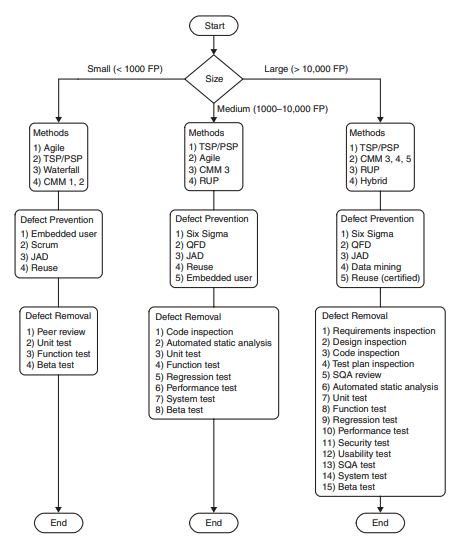
\includegraphics[width=0.8\textwidth]{jones-2010-development-methods}
    \caption[Development mehtods]{Development methods. Sorted by project size and success rates~\autocite[11]{jones_software_2010}}
    \label{fig:development-methods}
\end{figure}

The development methods displayed in \cref{fig:development-methods} are sorted according to their success rates.
As stated by~\textcite[10-12]{jones_software_2010}, projects with a size of less than 1000 function points are most likely to benefit from agile development methods.
The median size of function points is defined as 53 lines of JavaScript code by~\textcite{qsm_function_2009}.
Based on these findings, we will apply agile development methods during the development process as the project's size is not anticipated to grow beyond the aforementioned dimensions.

However, we will depart from the recommended defect prevention methods shown in~\cref{fig:development-methods} since embedded user reviews would mainly test the application’s frontend functionality.
Instead, the same goal can be achieved by applying Scrum methods and \gls{E2E} tests.

\subsection{End-to-end tests}\label{subsec:end-to-end-tests}

Since peer reviews are no feasible option for defect removal in a single-person project, we will employ E2E tests to check the application’s intended functionality and iteratively remove possible defects.
Also, in contrast to unit tests, \gls{E2E} tests provide the possibility to test entire workflows of the applications, such as the registration or voting process.

\section{Evaluation methods}\label{sec:evaluation-methods}

\subsection{Tests}\label{subsec:tests}
\subsection{Cryptocurrency transaction analysis}\label{subsec:crypto-currency-transaction-analysis}